\documentclass[11pt, A4paper,norsk]{article}
\usepackage[utf8]{inputenc}
\usepackage[T1]{fontenc}
\usepackage{babel}
\usepackage{amsmath}
\usepackage{amsfonts}
\usepackage{amsthm}
\usepackage[colorlinks]{hyperref}
\usepackage{listings}
\usepackage{color}
\usepackage{hyperref}
\usepackage{graphicx}
\usepackage{cite}

\definecolor{dkgreen}{rgb}{0,0.6,0}
\definecolor{gray}{rgb}{0.5,0.5,0.5}
\definecolor{daynineyellow}{rgb}{1.0,0.655,0.102}
\definecolor{url}{rgb}{0.1,0.1,0.4}

\lstset{frame=tb,
	language=Python,
	aboveskip=3mm,
	belowskip=3mm,
	showstringspaces=false,
	columns=flexible,
	basicstyle={\small\ttfamily},
	numbers=none,
	numberstyle=\tiny\color{gray},
	keywordstyle=\color{blue},
	commentstyle=\color{daynineyellow},
	stringstyle=\color{dkgreen},
	breaklines=true,
	breakatwhitespace=true,
	tabsize=3
}

\lstset{inputpath="C:/Users/Torstein/Documents/UiO/Fys2130/Python programmer"}
\hypersetup{colorlinks, urlcolor=url}

\author{Torstein Solheim Ølberg}
\title{Svar på Oblig nr. 1 i Fys2130}



%\lstinputlisting{Filnavn! type kodefil}
%\includegraphics[width=12.6cm,height=8cm]{"C:/Users/Torstein/Documents/UiO/Fys2130/Python programmer"/Filnavn! type png}



\begin{document}
\maketitle
	\begin{center}
\Large \textbf{Oppgaver}
	\end{center}









		\paragraph{2.}
			\begin{flushleft}
For at en kraft skal danne grunnlag for svigninger er den nødt til å være konservativ. Ellers vil ikke kraften kunne skifte retning slik at et objekt kan bevege seg fram og tilbake.
			\end{flushleft}









		\paragraph{4.}
			\begin{flushleft}
Periodetiden til en fjær og et lodd er $T = 2 \pi \sqrt{\frac{m}{k}}$ Denne tiden er ikke avhengig av tyngden til planeten, men utelukkende massen til objektet som ikke endres på månen. Derfor vil ikke periodetiden endre seg når vi tar med systemet opp på månen.
			\end{flushleft}









		\paragraph{5.}
			\begin{flushleft}
For frie svigninger til en pendel er uttrykket for periodetiden $T = 2 \pi \sqrt{\frac{L}{g}}$. Her ser vi at utrykket er avhengig av gravitasjonene til planeten, og derfor vil periodetiden til pendelen endre seg hvis den blir flyttet fra jorda til månen.
			\end{flushleft}
			









		\paragraph{7.}
			\begin{flushleft}
Ting som kan ødelegge for harmoniske svigninger er endringer eller krefter fra utenfor systemet som svinger. Som for eksempel en hånd som stopper eller dytter mot bevegelsen.
			\end{flushleft}










		\paragraph{9.}
			\begin{flushleft}
Plottet blir en sirkel.
			\end{flushleft}
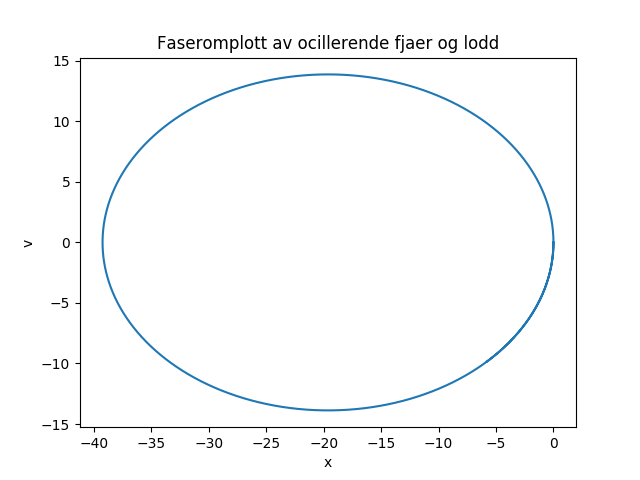
\includegraphics[width=12.6cm,height=8cm]{"C:/Users/Torstein/Documents/UiO/Fys2130/Python programmer"/Faserom_1.png}









		\paragraph{10.}
			\begin{flushleft}
Formen på plottet blir nå en halv sirkel delt vertikalt på midten, med en strek fra den ene siden av sirkelen til den andre.
			\end{flushleft}
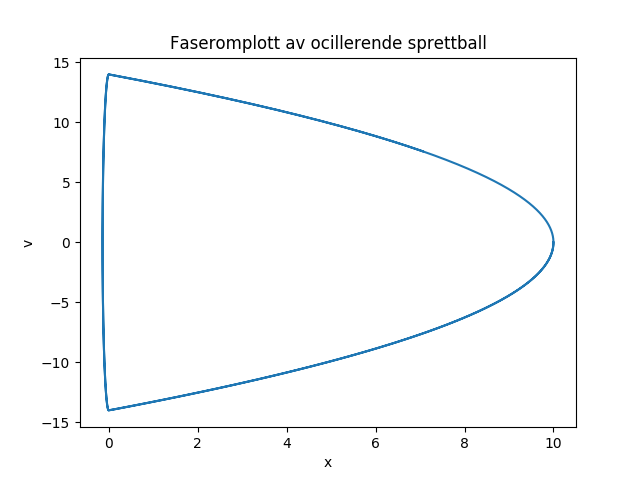
\includegraphics[width=12.6cm,height=8cm]{"C:/Users/Torstein/Documents/UiO/Fys2130/Python programmer"/Faserom_2.png}








		\paragraph{11.}
			\begin{flushleft}
Antar med svingetid det er snakk om periodetid, finner denne, og setter opp en matematisk model som kan uttrykke bevegelsen til loddet.
			\end{flushleft}
			\begin{gather}
F = mg \\
F = kx \\
kx = mg \\
k(-0.18m) = 0.1kg \cdot - 9.81m/s^2 \\
k = \frac{0.1 \cdot - 9.81}{- 0.18} = 9.45 kg/s^2 \\
\text{Vet fra tidligere hva som er uttrykket for periodetiden til en masse på en fjær.} \nonumber \\
\text{Dette kan utledes ved hjelp av en model for bevegelsen.} \nonumber \\
T = 2 \pi \sqrt{\frac{m}{k}} = 2 \cdot \pi \sqrt{\frac{0.1}{9.45}} = 0.646 sek \\
\text{Uttrykket for hele bevegelsen blir} \nonumber \\
x(t) = A \cos \left( \left(\omega = \frac{2 \pi}{T}\right) t - \phi \right) = - 0.08 \cos \left( 9.72111 t \right)
			\end{gather}
			\begin{flushleft}
Uttrykket for akselrasjonen med modelen over er $$a(t) = -A\omega^2 \cos(\omega t) = -0.08 \cdot 9.72111^2 \cos(\omega t)$$ og da er jo krafta akselrasjonen ganget med massen til loddet. $$F = ma = - m A \omega^2 \cos(\omega t) = - 0.1 \cdot 0.08 \cdot 9.72111^2 \cos(\omega t)$$ som er minst når $\omega t = 2 \pi$ og kraften blir da $F = - 0.1 \cdot 0.08 \cdot 9.72111^2 = -0.756$ og mest når kraften er lik det samme, bare med motsatt fortegn
			\end{flushleft}








		\paragraph{12.}
			\begin{gather}
x(t) = -A \cos \left( 2 \pi 0.4 t \right) \\
x(2) = 2.4 = -A \cos \left( 1.6 \pi \right) \Rightarrow A = \frac{- 2.4}{\cos(1.6 \pi)} = -7.7666 \\
a(2) = -A(0.8 \pi)^2 \cos (1.6\pi) = - 7.7666 \cdot 0.8^2 \cdot \pi^2 \cdot \cos (1.6\pi) \\
a(2) = - 15.160
			\end{gather}












		\paragraph{13.}
			\begin{gather}
E_T = E_p + E_k \\
E_T = \frac{1}{2}kA^2, E_p = \frac{1}{2} k x^2(t), \frac{1}{2} E_p \\
\frac{1}{2} k A^2 = E_p + \frac{1}{2} E_p = \frac{3}{2} E_p \\
\frac{1}{2} k A^2 = \frac{3}{4} k x(t)^2 \\
A^2 = \frac{3}{2} x(t)^2 \\
x(t) = \sqrt{\frac{2A^2}{3}}
			\end{gather}












		\paragraph{14.}
			\subparagraph{a)}
				\begin{gather*}
z(t) = A \cos(\omega t + \phi) = A \cos\left(\omega t + \frac{\pi}{6}\right) \\
z(t) = A\frac{e^{i\left( \omega t + \frac{\pi}{6} \right)} + e^{-i\left( \omega t + \frac{\pi}{6} \right)}}{2} \\
z(t) = A\frac{e^{i \omega t}e^{i\frac{\pi}{6}} + e^{-i \omega t}e^{-i\frac{\pi}{6}}}{2} \\
z(t) = A\frac{e^{i \omega t}(\frac{\sqrt{3}}{2} + \frac{i}{2}) + e^{-i \omega t}(\frac{\sqrt{3}}{2} - \frac{i}{2})}{2} \\
z(t) = A\frac{1}{4}((\sqrt{3} + i)(\cos(\omega t) + i\sin(\omega t)) + (\sqrt{3} - i)(\cos(\omega t) - i\sin(\omega t))) \\
z(t) = A \frac{1}{4}( \cos(\omega t) (\sqrt{3} + i + \sqrt{3} - i) + i\sin(\omega t) (\sqrt{3} + i - \sqrt{3} + i)) \\
z(t) = \frac{1}{4} A (2\sqrt{3} \cos(\omega t) - 2\sin(\omega t)) \\
z(t) = \frac{\sqrt{3}}{2} A \cos(\omega t) - \frac{1}{2} A \sin(\omega t)) \\
z(t) = \frac{\sqrt{3}}{2} A \cos(\omega t) - \frac{1}{2} A \sin(\omega t)) \\
z(t) = \frac{1.2}{2}(\sqrt{3}\cos(2\pi f t) - \sin(2\pi f t)) \\
z(t) = 0.6\left(\sqrt{3}\cos(6\pi t) - \sin(6\pi t)\right)
				\end{gather*}









			\subparagraph{b)}
				\begin{flushleft}
Bruker det jeg har funnet fra oppgave $a)$ på linje $3$.
				\end{flushleft}
				\begin{gather}
z(t) = \Re\left\{ 1.2 e^{i 6\pi t + i \frac{\pi}{6}} \right\}
				\end{gather}









		\paragraph{15.}
			\begin{gather*}
z(t) = A\sin(\omega t) + B\cos(\omega t) \\
C = \sqrt{A^2 + B^2} = \sqrt{1.2^2 + 0.7^2} = 1.38924 \\
\phi = -\arctan\left(\frac{B}{A}\right) = -\arctan\left(\frac{0.7}{1.2}\right) = -0.528074\\
z(t) =  1.38924 \cos(\omega t - 0.528074) \\
z(t) = \Re\left\{ 1.38924 e^{i (\omega t - 0.528074)} \right\}
			\end{gather*}








			\subparagraph{16.}
				\begin{gather*}
z(t) = \Re\{ (-5.8 + 2.2i)e^{i\omega t} \} = -5.8 \cos(\omega t) - 2.2 \sin(\omega t) \\
C = \sqrt{5.8^2 + 2.2^2} = 6.20322 \\
\phi = -\arctan\left( \frac{2.2}{5.8} \right) = - 0.362544 \\
z(t) = 6.20322 \cos(\omega t - 0.362544)
				\end{gather*}









			\subparagraph{19.}
				\begin{flushleft}
Energitapet på grunn av friksjonskraften er det samme som den deriverte av arbeidet kraften utfører med tanke på tid. $$\frac{dW}{dt} = F \cdot \dot{x} = F \cdot v = -b \cdot v^2$$ 
				\end{flushleft}
\end{document}